% !TEX encoding = UTF-8 Unicode
\documentclass[a4paper]{article}


\usepackage{color}
\usepackage{url}
\usepackage[T2A]{fontenc} % enable Cyrillic fonts
\usepackage[utf8]{inputenc} % make weird characters work
\usepackage{graphicx}

\usepackage[english,serbian]{babel}
%\usepackage[english,serbianc]{babel} %ukljuciti babel sa ovim opcijama, umesto gornjim, ukoliko se koristi cirilica

\usepackage[unicode]{hyperref}
\hypersetup{colorlinks,citecolor=green,filecolor=green,linkcolor=blue,urlcolor=blue}

\usepackage{listings}

%\newtheorem{primer}{Пример}[section] %ćirilični primer
\newtheorem{primer}{Primer}[section]

\definecolor{mygreen}{rgb}{0,0.6,0}
\definecolor{mygray}{rgb}{0.5,0.5,0.5}
\definecolor{mymauve}{rgb}{0.58,0,0.82}

\lstset{ 
  backgroundcolor=\color{white},   % choose the background color; you must add \usepackage{color} or \usepackage{xcolor}; should come as last argument
  basicstyle=\scriptsize\ttfamily,        % the size of the fonts that are used for the code
  breakatwhitespace=false,         % sets if automatic breaks should only happen at whitespace
  breaklines=true,                 % sets automatic line breaking
  captionpos=b,                    % sets the caption-position to bottom
  commentstyle=\color{mygreen},    % comment style
  deletekeywords={...},            % if you want to delete keywords from the given language
  escapeinside={\%*}{*)},          % if you want to add LaTeX within your code
  extendedchars=true,              % lets you use non-ASCII characters; for 8-bits encodings only, does not work with UTF-8
  firstnumber=1000,                % start line enumeration with line 1000
  frame=single,	                   % adds a frame around the code
  keepspaces=true,                 % keeps spaces in text, useful for keeping indentation of code (possibly needs columns=flexible)
  keywordstyle=\color{blue},       % keyword style
  language=Python,                 % the language of the code
  morekeywords={*,...},            % if you want to add more keywords to the set
  numbers=left,                    % where to put the line-numbers; possible values are (none, left, right)
  numbersep=5pt,                   % how far the line-numbers are from the code
  numberstyle=\tiny\color{mygray}, % the style that is used for the line-numbers
  rulecolor=\color{black},         % if not set, the frame-color may be changed on line-breaks within not-black text (e.g. comments (green here))
  showspaces=false,                % show spaces everywhere adding particular underscores; it overrides 'showstringspaces'
  showstringspaces=false,          % underline spaces within strings only
  showtabs=false,                  % show tabs within strings adding particular underscores
  stepnumber=2,                    % the step between two line-numbers. If it's 1, each line will be numbered
  stringstyle=\color{mymauve},     % string literal style
  tabsize=2,	                   % sets default tabsize to 2 spaces
  title=\lstname                   % show the filename of files included with \lstinputlisting; also try caption instead of title
}

\begin{document}

\title{Informacioni sistem za firmu Duma Group\\ \small{Seminarski rad u okviru kursa\\Informacioni sistemi\\ Matematički fakultet}}

\author{Miloš Miković, Anđela Križan, Milica Galjak, \\ Veronika Miljaković, Nikoleta Vukajlović}

%\date{9.~april 2015.}

\maketitle

\abstract{
%Ovde ide abstract
}

\tableofcontents

\newpage

\section{Uvod}

\section{Slučajevi upotrebe}

% Ovo je moj deo - Miloš

\subsection{Registrovanje i prijavljivanje korisnika}

\begin{figure}[htp]
    \centering
    
\includegraphics[width=8cm]{Slucaj upotrebe _Registrovanje.jpg}
    \caption{Dijagram slučaja upotrebe Registracija korisnika}
    \label{fig:Registracija}
\end{figure}

\subsubsection{Registrovanje korisnika}

\begin{itemize}
    \item Kratak opis:
        \begin{itemize}
            \item Korisnik se registruje kako bi mogao da koristi mogućnosti informacionog sistema Duma Group
        \end{itemize}
    \item Učesnici:
        \begin{itemize}
            \item Korisnik koji želi da koristi usluge Duma Group sistema
        \end{itemize}
    \item Preduslov:
        \begin{itemize}
            \item Korisnik mora da priloži tačne podatke pri registraciji
            \item Korisnik poseduje računar ili pametni telefon i pristup Internetu
            \item Sistem je u funkciji
        \end{itemize}
    \item Postuslov:
        \begin{itemize}
            \item Osoba je registrovana i otvoren joj je nalog za korišćenje sistema
        \end{itemize}
    \item Glavni tok:
        \begin{enumerate}
            \item  Korisnik otvara stranicu za registraciju odabirom određenog dugmeta na sajtu sistema
            \item Korisnik čita uslove korišćenja sistema 
            \item Korisnik prihvata postavljene uslove
            \item Korisnik popunjava formular unoseći tražene lične podatke. Kada zavši popunjavanje formulara pritiska dugme za registraciju
            \item Sistem obrađuje podatke i vrši validaciju
            \item Sistem kreira privremeni korisnički nalog
            \item Sistem šalje korisniku poruku na e-mail adresu unetu u formularu i čeka na potvrdu određeni period
            \item Korisnik proverava poštu i potvrđuje link za registraciju
            \item Sistem obeležava korisnički nalog kao aktivan
            \item Sistem obaveštava korisnika slanjem poruke na e-mail adresu korisnika da je nalog uspešno kreiran 
        \end{enumerate}
    \item Alternativni tok:
        \begin{itemize}
            \item Prilikom 2. koraka glavnog toka korisnik odbija uslove korišćenja sistema. Sistem obaveštava korisnika da mora da prihvati date uslove korišćenja i onemogućava dalji tok registracije dok korisnik ne prihvati date uslove.
            \item Prilikom koraka 5. ukoliko korisnik nije uneo ispravne podatke, sistem obaveštava korisnika i proces se nastavlja od koraka 4.
            \item Ukoliko korisnik nije prihvatio aktivacionu poruku u koraku 8. u određenom vremenskom periodu, sistem briše nalog i proces se završava.
            \item Ukoliko u koraku 8. korisnik nije primio aktivacionu poruku on obaveštava sistem da mu ponovo pošalje poruku
        \end{itemize}
    \item Dodatne informacije:
        \begin{itemize}
            \item Potrebni podaci za registraciju su korisničko ime, lozinka, potvrda lozinke, ime, prezime, e-mail naloga, e-mail za povratak naloga ako se desi da je korisnik zaboravi lozinku ili korisničko ime, datum rodjenja korisnika, pol korisnika
        \end{itemize}
\end{itemize}


\subsubsection{Prijavljivanje korisnika}

\begin{figure}[htp]
    \centering
    
\includegraphics[width=8cm]{Slucaj upotrebe _Prijavljivanje.jpg}
    \caption{Dijagram slučaja upotrebe Prijavljivanje korisnika}
    \label{fig:Prijavljivanje}
\end{figure}

\begin{itemize}
    \item Kratak opis:
        \begin{itemize}
            \item --
        \end{itemize}
    \item Učesnici:
        \begin{itemize}
            \item --
        \end{itemize}
    \item Preduslov:
        \begin{itemize}
            \item --
        \end{itemize}
    \item Postuslov:
        \begin{itemize}
            \item --
        \end{itemize}
    \item Glavni tok:
        \begin{enumerate}
            \item  --
        \end{enumerate}
    \item Alternativni tok:
        \begin{itemize}
            \item --
        \end{itemize}
    \item Dodatne informacije:
        \begin{itemize}
            \item --
        \end{itemize}
\end{itemize}


%Ovo je moj deo - Veronika

\subsection{Prenosivi bar}

%Ovde ide slika dijagrama i opis

\begin{figure}[htp]
    \centering
    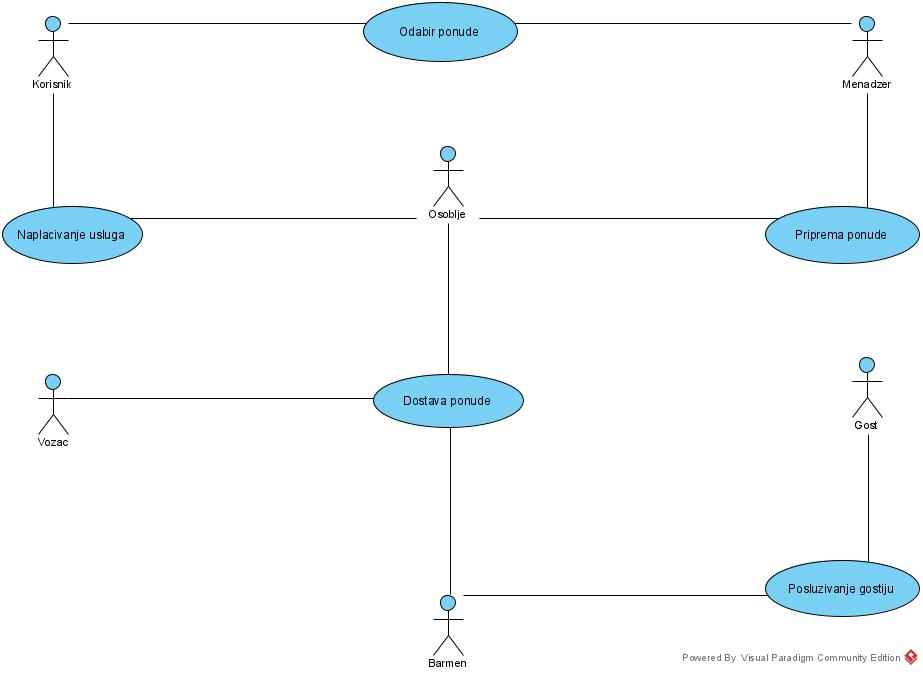
\includegraphics[width=8cm]{Slucaj upotrebe _ Prenosivi bar.jpg}
    \caption{Dijagram slučaja upotrebe Prenosivi bar}
    \label{fig:PrenosiviBar}
\end{figure}

\subsubsection{Odabir ponude}

\begin{itemize}
    \item Kratak opis:
        \begin{itemize}
            \item Korisnik bira odgovarajuću ponudu u skladu sa događajem za koji mu je usluga potrebna
        \end{itemize}
    \item Učesnici:
        \begin{itemize}
            \item Korisnik
            \item Menadžer za prenosivi bar
        \end{itemize}
    \item Preduslov:
        \begin{itemize}
            \item Korisnik se registrovao na sajt ili je pozvao telefonom
		    \item Na raspolaganju je spisak ponuda sa pratećim informacijama, slikama i snimcima
        \end{itemize}
    \item Postuslov:
        \begin{itemize}
            \item Korisnik je odabrao odgovarajuću ponudu
            \item Menadžer je prihvatio odabir i zabeležio potrebne detalje
        \end{itemize}
    \item Glavni tok:
        \begin{enumerate}
            \item  Korisnik se registruje na sajt
		    \item Opredeljuje se za uslugu ''Prenosivi bar''
		    \item Stupa u kontakt sa menadžerom za ovu uslugu
		    \item Korisnik objašnjava menadžeru kog je tipa događaj i za šta mu je potreban bar
		    \item Menadžer mu na mejl šalje ponudu iz ''Prenosivog bara'' sa pratećim informacijama o ceni, slikama i snimcima
		    \item Korisnik bira sadržaj koji želi iz ponude
		    \item Korisnik i menadžer dogovaraju detalje o datumu događaja, njegovom trajanju, da li je potrebno da na događaju bude i barmen, dodatnim zahtevima i upitima
		    \item Menadžer je primio sve potrebne detalje o događaju i rezervisao je odgovarajući datum
        \end{enumerate}
    \item Alternativni tok:
        \begin{itemize}
            \item Korak 5 : Sadržaj koji je korisnik odabrao nije dostupan. U tom slucaju menadžer zamoli korisnika da odabere nešto drugo iz ponude i uputi ga na ponudu koja je slična onoj koju je tražio
        \end{itemize}
\end{itemize}

\subsubsection{Priprema ponude}

\begin{itemize}
    \item Kratak opis:
        \begin{itemize}
            \item Menadžer za Prenosivi bar prenosi ponudu osoblju koje nakon toga priprema ono što je zahtevano
        \end{itemize}
    \item Učesnici:
        \begin{itemize}
            \item Menadžer za prenosivi bar
            \item Osoblje
        \end{itemize}
    \item Preduslov:
        \begin{itemize}
            \item Korisnik je odabrao svoju ponudu
		    \item Menadžer za prenosivi bar je prihvatio ponudu i zabeležio je	
        \end{itemize}
    \item Postuslov:
        \begin{itemize}
            \item Ponuda je pripremljena i spakovana za dostavu
        \end{itemize}
    \item Glavni tok:
        \begin{enumerate}
           \item Menadžer iznosi ponudu osoblju
		   \item Osoblje preuzima detalje o ponudi
	       \item Osoblje zaduženo za pripremu pića priprema odgovarajuću ponudu (donosi naručene flaše pića, čaše, slamčice, led i sve ostalo što je korisnik zahtevao)
	       \item Osoblje  zaduženo za nabavljanje prenosivog šanka, poslužaonika na kojima će se pića služiti i propratnih rekvizita za dekoraciju(cveće, table sa natpisima, baloni, ramovi za slikanje...) nabavlja ono što je potrebno za tip događaja koji korisnik pravi
	         \item Sav pripremljeni sadržaj se pakuje u prevozno sredstvo tako da bezbedno stigne na dogovorenu lokaciju
	        \item Sve je spremno za dostavu
        \end{enumerate}
\end{itemize}

\subsubsection{Dostava ponude}

\begin{itemize}
    \item Kratak opis:
        \begin{itemize}
            \item Ponuda je dovezena na potrebnu lokaciju i spremna za posluživanje
        \end{itemize}
    \item Učesnici:
        \begin{itemize}
            \item Vozač
            \item Osoblje
            \item Barmen
        \end{itemize}
    \item Preduslov:
        \begin{itemize}
            \item Sva potrebna roba je spakovana u prevozno sredstvo
		    \item Vozač je na raspolaganju	
        \end{itemize}
    \item Postuslov:
        \begin{itemize}
            \item Sve je postavljeno po dogovoru i događaj može da počne
        \end{itemize}
    \item Glavni tok:
        \begin{enumerate}
           \item Vozač dovozi robu i osoblje na dogovorenu adresu sat vremena pre početka događaja 
		    \item Osoblje montira prenosivi šank  
		    \item Osoblje ređa caše, flaše, poslužaonike na šank i dekoriše ga onako kako je dogovoreno sa korisnikom
		    \item Barmen dolazi na odgovarajuću adresu
	        \item Sve je spremno za početak događaja

        \end{enumerate}
    \item Alternativni tok:
        \begin{itemize}
            \item Korak 3 i 4: Korisnik se opredelio za opciju bez barmena koja podrazumeva da su pića vec sipana u caše i da će se gosti sami služiti. U tom slučaju potrebno je da osoblje pre početka dogadaja sipa pića u caše i poređa ih na poslužaonike.
        \end{itemize}
\end{itemize}

\subsubsection{Posluživanje gostiju}

\begin{itemize}
    \item Kratak opis:
        \begin{itemize}
            \item Gosti dolaze do šanka gde im barmen sipa pića i pravi odgovarajuće koktele 
        \end{itemize}
    \item Učesnici:
        \begin{itemize}
            \item Gosti
            \item Barmen
        \end{itemize}
    \item Preduslov:
        \begin{itemize}
            \item Barmen je došao na adresu
		    \item Barmenu su dostupne čaše i odgovarajuća pića i dodaci za određene koktele	
        \end{itemize}
    \item Postuslov:
        \begin{itemize}
            \item Svi gosti su usluženi na odgovarajući način
        \end{itemize}
    \item Glavni tok:
        \begin{enumerate}
           \item Gost dolazi do šanka
		   \item Gost naručuje jedno ili više pića
		   \item Barmen pravi pića i daje ih gostu
		   \item Gost preuzima pica
		  \end{enumerate}
		\textit{Koraci se ponavljaju za svakog gosta koji priđe šanku sve do kraja događaja}
	
    \item Alternativni tok:
        \begin{itemize}
            \item Korak 1-4 : Barmen je trenutno zauzet pripremanjem pića za nekog drugog gosta. U tom slucaju potrebno je malo sačekati da se barmen oslobodi i onda zahtevati piće od njega.
	      \item	Korak 3 : Piće koje korisnik traži je u međuvremenu popijeno. U tom slučaju barmen preporučuje gostu neka druga pića koja su dostupna i korisnik bira jedno od njih.

        \end{itemize}
\end{itemize}

\subsubsection{Naplaćivanje usluga}

\begin{itemize}
    \item Kratak opis:
        \begin{itemize}
            \item Po završetku događaja osoblje naplaćuje uslugu, posprema bar, pakuje svoje stvari i odlazi sa mesta događaja
        \end{itemize}
    \item Učesnici:
        \begin{itemize}
            \item Osoblje
            \item Korisnik
        \end{itemize}
    \item Preduslov:
        \begin{itemize}
            \item Događaj je završen
        \end{itemize}
    \item Postuslov:
        \begin{itemize}
            \item Usluga je plaćena
		    \item Bar je pospremljen i spakovan
		    \item Osoblje je otišlo sa mesta događaja
        \end{itemize}
    \item Glavni tok:
        \begin{enumerate}
          \item Osoblje čisti i rasprema šank
		  \item Osoblje pakuje čaše, flaše i prateće rekvizite koje su koristili na dogadaju
		  \item Osoblje ispostavlja korisniku račun usluge
		  \item Korisnik isplaćuje uslugu
		  \item Osoblje odlazi sa mesta događaja
		  \end{enumerate}
    
\end{itemize}

\subsection{Rad sa zaposlenima u firmi}

\subsubsection{Registracija zaposlenih}

\begin{figure}[htp]
    \centering
    \includegraphics[width=8cm]{Registracija_zaposlenog.jpg}
    \caption{Dijagram slučaja upotrebe Registracija zaposlenog}
    \label{fig:RegistracijaZ}
\end{figure}

\begin{itemize}
    \item Kratak opis: 
    \begin{itemize}
        \item Zaposleni u firmi se registruje na sistem Douma Group firme popunjavanjem osnovnih podataka. Sistem izvršava validaciju i vraća potvrdu o registraciji, ukoliko je uspešna.
    \end{itemize}
    \item Učesnici:
        \begin{itemize}
        \item Neregistrovani zaposleni
    \end{itemize}
    \item Preduslovi:
        \begin{itemize}
            \item Osoba koja pokušava da se registruje je zaposlena u firmi
            \item Zaposleni ima pristup internetu, računaru ili pametnom telefonu
            \item Sistem je u funkciji
        \end{itemize}
    \item Postuslovi:
        \begin{itemize}
            \item Zaposleni je registrovan u sistem i dobija informaciju o tome
        \end{itemize}
    \item Glavni tok:
        \begin{enumerate}
            \item Zaposleni pristupa stranici za registraciju
            \item Zaposleni popunjava formular o sopstvenim podacima 
            \item Sistem vrši validaciju podataka 
            \item Sistem zaposlenom šalje mejl sa privremenim linkom za potvrdu
            \item Zaposleni potvrđuje link za potvrdu i čeka potvrdu o registracija
            \item Sistem potvrđuje nalog kao aktivan
            \item Sistem obaveštava korisnika da je uspešno registrovan 
        \end{enumerate}
    \item Alternativni tokovi:
        \begin{itemize}
            \item Neuspešna validacija - Ukoliko zaposleni nije uneo ispravne podatke, sistem obaveštava korisnika o tome i proces se nastavlja u koraku 2.
            \item Link za registraciju nije stigao - Ukoliko u koraku 5 zaposlenom nije stigao mejl za potvrdu, on obaveštava sistem kako bi mu poslao novi link za potvrdu. Proces se nastavlja u koraku 4.
            \item Link za registraciju je istekao - Ukoliko u koraku 5, zaposleni ne potvrdi registraciju u određenom periodu, sistem briše nalog i proces se završava.
        \end{itemize}
    \item Dodatne informacije:
        \begin{itemize}
            \item Neophodni podaci za prijavu su ime, prezime, e-mail adresa, pozicija zaposlenog u firmi, lozinka i potvrđena lozinka.
        \end{itemize}
\end{itemize}

\subsubsection{Otpuštanje zaposlenog}

\begin{figure}[htp]
    \centering
    \includegraphics[width=8cm]{Prekid_radnog_odnosa.jpg}
    \caption{Dijagram slučaja upotrebe Prekid radnog odnosa}
    \label{fig:Prekid}
\end{figure}

\begin{itemize}
    \item Kratak opis: 
    \begin{itemize}
        \item Prekida se radni odnos sa zaposlenim.
    \end{itemize}
    \item Učesnici:
        \begin{itemize}
        \item Zaposleni
        \item CEO menadžer
    \end{itemize}
    \item Preduslovi:
        \begin{itemize}
            \item Korisnici nisu zadovoljni uslugom koju je zaposleni pružio
            \item Poslodavac nije zadovoljan radom zaposlenog
            \item Zaposleni nije zadovoljan uslovima rada
        \end{itemize}
    \item Postuslovi:
        \begin{itemize}
            \item Zaposleni dobija otkaz i obrisan mu je nalog
        \end{itemize}
    \item Glavni tok:
        \begin{enumerate}
            \item CEO menadžer pokreće postupak prekida radnog odnosa sa zaposlenim
            \item Zaposleni dobija otkaz
            \item Korisnički nalog je obrisan
        \end{enumerate}
    \item Alternativni tokovi:
        \begin{itemize}
            \item Prilikom koraka 2, zaposleni svojevoljno daje otkaz
        \end{itemize}
\end{itemize}

\end{document}
























